
\documentclass[journal,10pt]{IEEEtran}
\usepackage{graphicx}
\usepackage{chngpage}
\usepackage{multirow}
\newcommand{\subparagraph}{}
% \usepackage [english]{babel}
% \usepackage [autostyle, english = american]{csquotes}
\usepackage{pgfplots}
\usepackage{mathtools}
\usepackage{multicol}
\usepackage{titlesec}
\usepackage{gensymb}
\usepackage[justification=centering]{caption}
\usepackage{amsmath}
\usepackage{algorithm}
\usepackage[noend]{algpseudocode}
\usepackage{url}
\usepackage[final]{pdfpages}
%\usepackage{appendix}
\usepackage{float}
\usepackage{subfig}
 \usepackage[
    backend=biber,
    style=ieee,
  ]{biblatex}
\addbibresource{main.bib}
\usepackage[margin=0.75in]{geometry} % see geometry.pdf on how to lay out the page. There's lots.
\geometry{a4paper} % or letter or a5paper or ... etc
\setlength{\parskip}{0.5
em}








% *** GRAPHICS RELATED PACKAGES ***
%
\ifCLASSINFOpdf
  % \usepackage[pdftex]{graphicx}
  % declare the path(s) where your graphic files are
  % \graphicspath{{../pdf/}{../jpeg/}}
  % and their extensions so you won't have to specify these with
  % every instance of \includegraphics
  % \DeclareGraphicsExtensions{.pdf,.jpeg,.png}
\else
  % or other class option (dvipsone, dvipdf, if not using dvips). graphicx
  % will default to the driver specified in the system graphics.cfg if no
  % driver is specified.
  % \usepackage[dvips]{graphicx}
  % declare the path(s) where your graphic files are
  % \graphicspath{{../eps/}}
  % and their extensions so you won't have to specify these with
  % every instance of \includegraphics
  % \DeclareGraphicsExtensions{.eps}
\fi
% graphicx was written by David Carlisle and Sebastian Rahtz. It is
% required if you want graphics, photos, etc. graphicx.sty is already
% installed on most LaTeX systems. The latest version and documentation
% can be obtained at: 
% http://www.ctan.org/tex-archive/macros/latex/required/graphics/
% Another good source of documentation is "Using Imported Graphics in
% LaTeX2e" by Keith Reckdahl which can be found at:
% http://www.ctan.org/tex-archive/info/epslatex/
%
% latex, and pdflatex in dvi mode, support graphics in encapsulated
% postscript (.eps) format. pdflatex in pdf mode supports graphics
% in .pdf, .jpeg, .png and .mps (metapost) formats. Users should ensure
% that all non-photo figures use a vector format (.eps, .pdf, .mps) and
% not a bitmapped formats (.jpeg, .png). IEEE frowns on bitmapped formats
% which can result in "jaggedy"/blurry rendering of lines and letters as
% well as large increases in file sizes.
%
% You can find documentation about the pdfTeX application at:
% http://www.tug.org/applications/pdftex





% *** MATH PACKAGES ***
%
%\usepackage[cmex10]{amsmath}
% A popular package from the American Mathematical Society that provides
% many useful and powerful commands for dealing with mathematics. If using
% it, be sure to load this package with the cmex10 option to ensure that
% only type 1 fonts will utilized at all point sizes. Without this option,
% it is possible that some math symbols, particularly those within
% footnotes, will be rendered in bitmap form which will result in a
% document that can not be IEEE Xplore compliant!
%
% Also, note that the amsmath package sets \interdisplaylinepenalty to 10000
% thus preventing page breaks from occurring within multiline equations. Use:
%\interdisplaylinepenalty=2500
% after loading amsmath to restore such page breaks as IEEEtran.cls normally
% does. amsmath.sty is already installed on most LaTeX systems. The latest
% version and documentation can be obtained at:
% http://www.ctan.org/tex-archive/macros/latex/required/amslatex/math/





% *** SPECIALIZED LIST PACKAGES ***
%
%\usepackage{algorithmic}
% algorithmic.sty was written by Peter Williams and Rogerio Brito.
% This package provides an algorithmic environment fo describing algorithms.
% You can use the algorithmic environment in-text or within a figure
% environment to provide for a floating algorithm. Do NOT use the algorithm
% floating environment provided by algorithm.sty (by the same authors) or
% algorithm2e.sty (by Christophe Fiorio) as IEEE does not use dedicated
% algorithm float types and packages that provide these will not provide
% correct IEEE style captions. The latest version and documentation of
% algorithmic.sty can be obtained at:
% http://www.ctan.org/tex-archive/macros/latex/contrib/algorithms/
% There is also a support site at:
% http://algorithms.berlios.de/index.html
% Also of interest may be the (relatively newer and more customizable)
% algorithmicx.sty package by Szasz Janos:
% http://www.ctan.org/tex-archive/macros/latex/contrib/algorithmicx/




% *** ALIGNMENT PACKAGES ***
%
%\usepackage{array}
% Frank Mittelbach's and David Carlisle's array.sty patches and improves
% the standard LaTeX2e array and tabular environments to provide better
% appearance and additional user controls. As the default LaTeX2e table
% generation code is lacking to the point of almost being broken with
% respect to the quality of the end results, all users are strongly
% advised to use an enhanced (at the very least that provided by array.sty)
% set of table tools. array.sty is already installed on most systems. The
% latest version and documentation can be obtained at:
% http://www.ctan.org/tex-archive/macros/latex/required/tools/


% IEEEtran contains the IEEEeqnarray family of commands that can be used to
% generate multiline equations as well as matrices, tables, etc., of high
% quality.




% *** SUBFIGURE PACKAGES ***
%\ifCLASSOPTIONcompsoc
%  \usepackage[caption=false,font=normalsize,labelfont=sf,textfont=sf]{subfig}
%\else
%  \usepackage[caption=false,font=footnotesize]{subfig}
%\fi
% subfig.sty, written by Steven Douglas Cochran, is the modeuion replacement
% for subfigure.sty, the latter of which is no longer maintained and is
% incompatible with some LaTeX packages including fixltx2e. However,
% subfig.sty requires and automatically loads Axel Sommerfeldt's caption.sty
% which will override IEEEtran.cls' handling of captions and this will result
% in non-IEEE style figure/table captions. To prevent this problem, be sure
% and invoke subfig.sty's "caption=false" package option (available since
% subfig.sty version 1.3, 2005/06/28) as this is will preserve IEEEtran.cls
% handling of captions.
% Note that the Computer Society format requires a larger sans serif font
% than the serif footnote size font used in traditional IEEE formatting
% and thus the need to invoke different subfig.sty package options depending
% on whether compsoc mode has been enabled.
%
% The latest version and documentation of subfig.sty can be obtained at:
% http://www.ctan.org/tex-archive/macros/latex/contrib/subfig/




% *** FLOAT PACKAGES ***
%
%\usepackage{fixltx2e}
% fixltx2e, the successor to the earlier fix2col.sty, was written by
% Frank Mittelbach and David Carlisle. This package corrects a few problems
% in the LaTeX2e kernel, the most notable of which is that in current
% LaTeX2e releases, the ordering of single and double column floats is not
% guaranteed to be preserved. Thus, an unpatched LaTeX2e can allow a
% single column figure to be placed prior to an earlier double column
% figure. The latest version and documentation can be found at:
% http://www.ctan.org/tex-archive/macros/latex/base/


%\usepackage{stfloats}
% stfloats.sty was written by Sigitas Tolusis. This package gives LaTeX2e
% the ability to do double column floats at the bottom of the page as well
% as the top. (e.g., "\begin{figure*}[!b]" is not normally possible in
% LaTeX2e). It also provides a command:
%\fnbelowfloat
% to enable the placement of footnotes below bottom floats (the standard
% LaTeX2e kernel puts them above bottom floats). This is an invasive package
% which rewrites many portions of the LaTeX2e float routines. It may not work
% with other packages that modify the LaTeX2e float routines. The latest
% version and documentation can be obtained at:
% http://www.ctan.org/tex-archive/macros/latex/contrib/sttools/
% Do not use the stfloats baselinefloat ability as IEEE does not allow
% \baselineskip to stretch. Authors submitting work to the IEEE should note
% that IEEE rarely uses double column equations and that authors should try
% to avoid such use. Do not be tempted to use the cuted.sty or midfloat.sty
% packages (also by Sigitas Tolusis) as IEEE does not format its papers in
% such ways.
% Do not attempt to use stfloats with fixltx2e as they are incompatible.
% Instead, use Morten Hogholm'a dblfloatfix which combines the features
% of both fixltx2e and stfloats:
%
% \usepackage{dblfloatfix}
% The latest version can be found at:
% http://www.ctan.org/tex-archive/macros/latex/contrib/dblfloatfix/




%\ifCLASSOPTIONcaptionsoff
%  \usepackage[nomarkers]{endfloat}
% \let\MYoriglatexcaption\caption
% \renewcommand{\caption}[2][\relax]{\MYoriglatexcaption[#2]{#2}}
%\fi
% endfloat.sty was written by James Darrell McCauley, Jeff Goldberg and 
% Axel Sommerfeldt. This package may be useful when used in conjunction with 
% IEEEtran.cls'  captionsoff option. Some IEEE journals/societies require that
% submissions have lists of figures/tables at the end of the paper and that
% figures/tables without any captions are placed on a page by themselves at
% the end of the document. If needed, the draftcls IEEEtran class option or
% \CLASSINPUTbaselinestretch interface can be used to increase the line
% spacing as well. Be sure and use the nomarkers option of endfloat to
% prevent endfloat from "marking" where the figures would have been placed
% in the text. The two hack lines of code above are a slight modification of
% that suggested by in the endfloat docs (section 8.4.1) to ensure that
% the full captions always appear in the list of figures/tables - even if
% the user used the short optional argument of \caption[]{}.
% IEEE papers do not typically make use of \caption[]'s optional argument,
% so this should not be an issue. A similar trick can be used to disable
% captions of packages such as subfig.sty that lack options to turn off
% the subcaptions:
% For subfig.sty:
% \let\MYorigsubfloat\subfloat
% \renewcommand{\subfloat}[2][\relax]{\MYorigsubfloat[]{#2}}
% However, the above trick will not work if both optional arguments of
% the \subfloat command are used. Furthermore, there needs to be a
% description of each subfigure *somewhere* and endfloat does not add
% subfigure captions to its list of figures. Thus, the best approach is to
% avoid the use of subfigure captions (many IEEE journals avoid them anyway)
% and instead reference/explain all the subfigures within the main caption.
% The latest version of endfloat.sty and its documentation can obtained at:
% http://www.ctan.org/tex-archive/macros/latex/contrib/endfloat/
%
% The IEEEtran \ifCLASSOPTIONcaptionsoff conditional can also be used
% later in the document, say, to conditionally put the References on a 
% page by themselves.




% *** PDF, URL AND HYPERLINK PACKAGES ***
%
%\usepackage{url}
% url.sty was written by Donald Arseneau. It provides better support for
% handling and breaking URLs. url.sty is already installed on most LaTeX
% systems. The latest version and documentation can be obtained at:
% http://www.ctan.org/tex-archive/macros/latex/contrib/url/
% Basically, \url{my_url_here}.




% *** Do not adjust lengths that control margins, column widths, etc. ***
% *** Do not use packages that alter fonts (such as pslatex).         ***
% There should be no need to do such things with IEEEtran.cls V1.6 and later.
% (Unless specifically asked to do so by the journal or conference you plan
% to submit to, of course. )


% correct bad hyphenation here
\hyphenation{op-tical net-works semi-conduc-tor}

\graphicspath{{imgs/}{}}
\begin{document}
%
% paper title
% Titles are generally capitalized except for words such as a, an, and, as,
% at, but, by, for, in, nor, of, on, or, the, to and up, which are usually
% not capitalized unless they are the first or last word of the title.
% Linebreaks \\ can be used within to get better formatting as desired.
% Do not put math or special symbols in the title.
\title{ELEN 4020 Lab 1: Tensor Arithmetic}
%
%
% author names and IEEE memberships
% note positions of commas and nonbreaking spaces ( ~ ) LaTeX will not break
% a structure at a ~ so this keeps an author's name from being broken across
% two lines.
% use \thanks{} to gain access to the first footnote area
% a separate \thanks must be used for each paragraph as LaTeX2e's \thanks
% was not built to handle multiple paragraphs
%
%\onecolumn
\author{Junaid Dawood (1094837), Xongile Nghatsane (1110680), Marissa van Wyngaardt (719804)}% <-this % stops a space



\maketitle

% As a general rule, do not put math, special symbols or citations
% in the abstract or keywords.

\begin{abstract}
This report discusses the basic properties of matrix multiplication as well as an attempt to formalise the process of 3D vector multiplication. These are both done with reference to a C implementation of these algorithms.
\end{abstract}

\IEEEpeerreviewmaketitle

\section{Introduction}

This document discusses the implementation of some simple tensor arithmetic operations in C. This extends to the description of the implemented algorithms, significant features, and pseudocode of said algorithms.

\section{Tensor Structs and Helper Functions}

A \textit{struct} is implemented to represent rank 2 and rank 3 tensors. This \textit{struct} stores the dimensions of the tensor as well as the actual N dimensional array which holds the contents of the tensor. In the case of a rank 2 tensor, the \textit{struct} holds a row and column count as well as an \textit{int**} representing the matrix. With rank 3 tensors, an additional height variable is present, and the \textit{int**} is naturally replaced by a \textit{int***}.

Additional helper functions for the initialisation of the contents of the tensor and the freeing of memory dynamically allocated for their content are implemented. The helper functions, as well as the arithmetic functions, take pointers to tensor \textit{structs} as arguments.


\section{Implementation of Rank 3 Tensor Multiplication}
The concept of 3D vector multiplication is not well defined. In comparison, 2D vector(matrix) multiplication is a well defined and commonly used mathematical procedure. In addition, conformity for matrix multiplication is well defined. That is, two matrices will only have a defined product if the number of columns in $A$ is equal to the number of rows in $B$; in the case of $A \times B = C$. 

Hence, the challenge with 3D vector multiplication is to set up a set of rules for doing so, such that the process is internally consistent. This includes the process of defining conformity for 3D vector products i.e. what dimensional equality must there be for the product of two 3D vectors to exist. One such formalization is present in \cite{solo2010multidimensional}.

The proposed definition of 3D vector multiplication is to compute a partial matrix multiplication of `column' and `row' matrices for each $(i,j,k)$ in the resultant 3D vector. The `row' matrix is defined by fixing the height value, the $i$ coordinate in $A$. Similarly, if the row value, the $j$ coordinate in $B$, is fixed, this will yield the `column' matrix. 

For each $(i,j,k)$ in the resultant 3D vector, it is required that a partial multiplication of the `row' and `column' matrices be done. The procedure has been implemented such that each $(i,j,k)$ will be equivalent to an element on the diagonal of the product of the `row' and `column' matrices. That is, for each $(i,j,k)$ in the resultant 3D vector the row vector in $A$ at $(i,k,:)$ will be multiplied by the column vector at $(:,j,k)$ in $B$.

The diagram below is provided to give a visualisation of the process decided upon.

\begin{figure}[H]
    \centering
    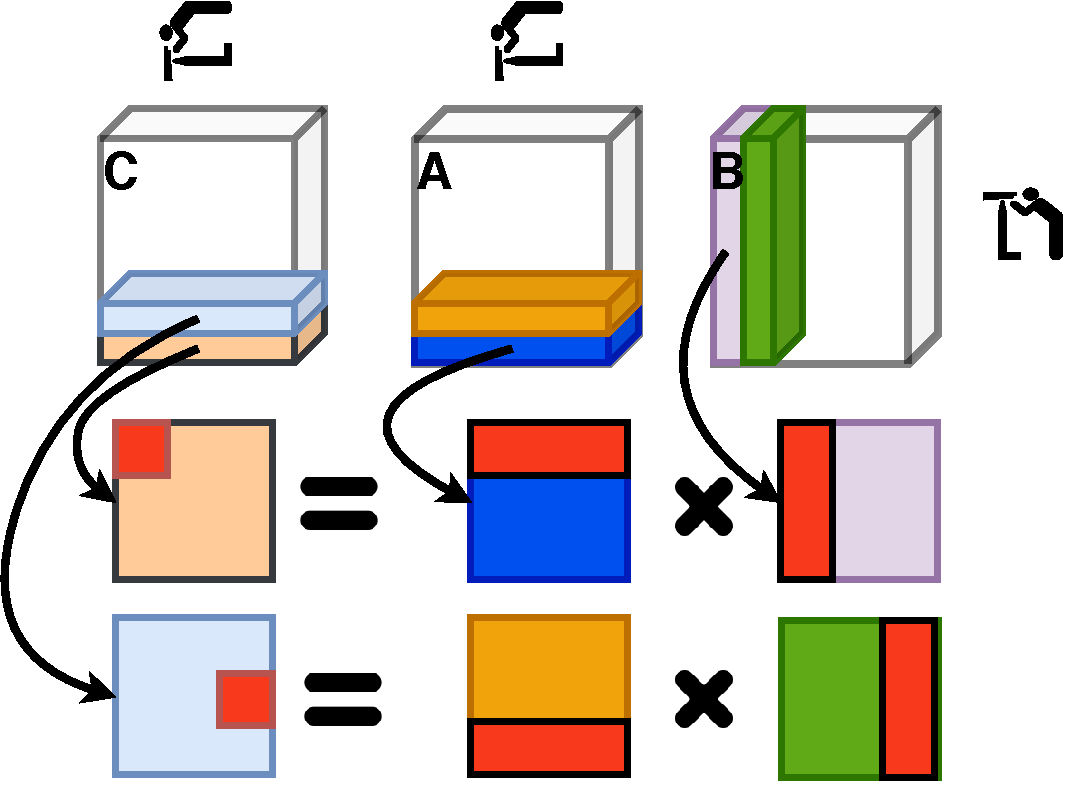
\includegraphics[width=0.5\textwidth]{export.pdf}
    \caption{3D Vector Multiplication Visualisation.}
    \label{}
\end{figure}


\subsubsection{Conformity}

As per the definition of 3D vector given above, there must be conformity between the `column' matrices and the `row' matrices as per typical matrix multiplication rules. The current implementation relies on cube 3D vectors only i.e. ones which are equal in all dimensions, and returns errors when this is not the case.

\section{Additional Implementation}
The concept of using a one dimensional array for the purpose of the general representation of an N dimensional array was experimented with. It is known that the naive matrix multiplication algorithm possesses $O(n^3)$ complexity, although there exists some sub-cubic implementations. For example, the Coppersmith-Winograd algorithm, the fastest algorithm currently known, achieves $O{n^{2.3728639}}$ complexity \cite{copper}.

Whilst the flattening of N dimensional arrays does not change the asymptotic complexity, it does offer potentially easier parallelisation of the matrix arithmetic procedures. At the very least, this collapses the process of matrix addition to a single \textit{for} loop.

\clearpage

\section{Conclusion}

A discussion of matrix multiplication methodologies has been presented, alongside a formalisation of the process of 3D vector multiplication. The drawbacks of the naive implementation, as well as more efficient alternatives have also been discussed. Some thought was also given on the process of parallelising the algorithm(s), as indicated.

\renewcommand*{\bibfont}{\small}

\printbibliography

\clearpage

\onecolumn
\section*{Pseudocode}
\pagenumbering{gobble}

\begin{algorithm}
\caption{Rank 2 Tensor Addition}\label{euclid}
\begin{algorithmic}[1]
\Function{rank2TensorAdd}{rank2Tensor t1, rank2Tensor t2}
\State $\textit{t1} \gets \textit{first rank 2 tensor}$
\State $t2 \gets \textit{second rank 2 tensor}$

\If {$t1 dimensions = t2 dimensions$} \Return ErrorResult
\EndIf
\For{i=0..t1.rows}
\For{j=0..t1.columns}

Result[i][j]=t1[i][j]+t2[i][j]

\EndFor
\EndFor
\Return Result


\EndFunction
\end{algorithmic}
\end{algorithm}

\begin{algorithm}
\caption{Rank 2 Tensor Multiplication}\label{euclid}
\begin{algorithmic}[1]
\Function{rank2TensorMult}{rank2Tensor t1, rank2Tensor t2}
\State $\textit{t1} \gets \textit{first rank 2 tensor}$
\State $t2 \gets \textit{second rank 2 tensor}$

\If {$t1.columns \neq t2.rows$} \Return ErrorResult
\EndIf
Result.rows=t1.rows
Results.columns=t2.columns
\For{i=0..t1.rows}
\For{j=0..t2.columns}
Sum = 0
\For{}
sum += t1[i][k]*t2[k][j]
\EndFor
Result[i][j]=sum


\EndFor
\EndFor
\Return Result


\EndFunction
\end{algorithmic}
\end{algorithm}


\begin{algorithm}
\caption{Rank 3 Tensor Addition}\label{euclid}
\begin{algorithmic}[1]
\Function{rank3TensorAdd}{rank3Tensor t1, rank3Tensor t2}
\State $\textit{t1} \gets \textit{first rank 3 tensor}$
\State $t2 \gets \textit{second rank 3 tensor}$

\If {$t1 dimensions = t2 dimensions$} \Return ErrorResult
\EndIf
\For{i=0..t1.height}
\For{j=0..t1.rows}
\For{k=0..t1.columns}

Result[i][j][k]=t1[i][j][k]+t2[i][j][k]


\EndFor
\EndFor
\EndFor
\Return Result


\EndFunction
\end{algorithmic}
\end{algorithm}


\begin{algorithm}
\caption{Rank 3 Tensor Multiplication}\label{euclid}
\begin{algorithmic}[1]
\Function{rank3TensorMult}{rank3Tensor t1, rank3Tensor t2}
\State $\textit{t1} \gets \textit{first rank 3 tensor}$
\State $t2 \gets \textit{second rank 3 tensor}$

\If {$t1.columns \neq t2.rows$} \Return ErrorResult
\EndIf
Result.rows=t1.rows
Result.columns=t2.columns
\For{i=0..Result.height}
\For{j=0..Result.rows}
\For{k=0..Result.columns}
Sum = 0
\For{l=0..t1.columns}
sum += t1[i][k][l]*t2[height-1-l][j][k]
\EndFor
Result[i][j][k]=sum


\EndFor
\EndFor
\EndFor
\Return Result


\EndFunction
\end{algorithmic}
\end{algorithm}




\clearpage

\newrefsection
\pagenumbering{arabic}
\onecolumn 
%\setlength{\parskip}{0.6em}




\ifCLASSOPTIONcaptionsoff
  \newpage
\fi



% trigger a \newpage just before the given reference
% number - used to balance the columns on the last page
% adjust value as needed - may need to be readjusted if
% the document is modified later
%\IEEEtriggeratref{8}
% The "triggered" command can be changed if desired:
%\IEEEtriggercmd{\enlargethispage{-5in}}

% references section

% can use a bibliography generated by BibTeX as a .bbl file
% BibTeX documentation can be easily obtained at:
% http://www.ctan.org/tex-archive/biblio/bibtex/contrib/doc/
% The IEEEtran BibTeX style support page is at:
% http://www.michaelshell.org/tex/ieeetran/bibtex/
%\bibliographystyle{IEEEtran}
% argument is your BibTeX string definitions and bibliography database(s)
%\bibliography{IEEEabrv,../bib/paper}
%
% <OR> manually copy in the resultant .bbl file
% set second argument of \begin to the number of references
% (used to reserve space for the reference number labels box)
%\begin{thebibliography}{1}

%\bibitem{IEEEhowto:kopka}

% H.~Kopka and P.~W. Daly, \emph{A Guide to \LaTeX}, 3rd~ed.\hskip 1em plus
%   0.5em minus 0.4em\relax Harlow, England: Addison-Wesley, 1999.

%\end{thebibliography}

% biography section
% 
% If you have an EPS/PDF photo (graphicx package needed) extra braces are
% needed around the contents of the optional argument to biography to prevent
% the LaTeX parser from getting confused when it sees the complicated
% \includegraphics command within an optional argument. (You could create
% your own custom macro containing the \includegraphics command to make things
% simpler here.)
%\begin{IEEEbiography}[{\includegraphics[width=1in,height=1.25in,clip,keepaspectratio]{mshell}}]{Michael Shell}
% or if you just want to reserve a space for a photo:

% \begin{IEEEbiography}
% Biography text here.
% \end{IEEEbiography}

% if you will not have a photo at all:
% \begin{IEEEbiographynophoto}{John Doe}
% Biography text here.
% \end{IEEEbiographynophoto}

% insert where needed to balance the two columns on the last page with
% biographies
%\newpage

% \begin{IEEEbiographynophoto}{Jane Doe}
% Biography text here.
% \end{IEEEbiographynophoto}

% You can push biographies down or up by placing
% a \vfill before or after them. The appropriate
% use of \vfill depends on what kind of text is
% on the last page and whether or not the columns
% are being equalized.

%\vfill

% Can be used to pull up biographies so that the bottom of the last one
% is flush with the other column.
%\enlargethispage{-5in}



% that's all folks
\end{document}